\section{Results}
\label{sec:results}
The results from the experiments in the project report \cite{project-report},
showed that the query expansion implementation had about 2 times longer latency compared to the baseline implementation.
The latency was measured from the request left the user to the response from the server arrived.

All the results show that the first request is often the slowest.
After the initial request,
the response is cached by Lucene and makes all the subsequent requests a lot faster.

\subsection{Lucene Results}
The query expansion implementation was evaluated by measuring the time from the Java program sends the request to Lucene index,
until a result is returned from the index.
Before starting the tests, the index cache was prewarmed using the terms \texttt{square} and \texttt{insta}.
The prewarming was done sending 10,000 requests to the Lucene index.
5,000 of the requests were multi term queries and the other 5,000 requests were query expansion queries.
With half of the results each, both term types will be present in Lucene's cache.
Figure \ref{fig:lucene-results} displays the measured response times from the Lucene experiments.
The red line is response times from the query expansion search, and the blue line displays the baseline query response times.
Even though the measured response times is within the requirement for interactive applications,
the experiment is not a good indicator for how it would have performed in a real world environment.
More interesting is how many times slower query expansion is compared to the baseline query.
When the result size contains 10 results,
query expansion is more than 3 times slower compared to the baseline query,
and it increases to more than 5 times slower when the result size is 200.
This means that the response times are increasing faster with query expansion compared to the baseline query.

\begin{figure}[h!]
  \centering 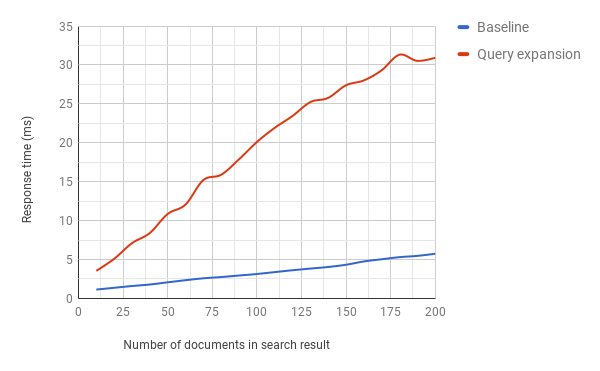
\includegraphics[width=1\linewidth]{img/lucene-results.png}
  \caption{Response times from the Lucene implementation with varying result size.}
  \label{fig:lucene-results}
\end{figure}

\subsection{Elasticsearch Experiment Results}
As mentioned earlier,
the Elasticsearch plugin is evaluated by measuring the response time from the client sends the request until the response arrives at the client.
The response times were measured using a command line tool called ApacheBench (\texttt{ab}) \cite{apache-benchmark},
and the actual command used can be found in appendix \ref{ap:apache-benchmark}.
\texttt{ab} collects min, average, median and the max response time for all the responses.
The results also includes information about the different parts of the response time:
connection time, processing time and waiting time.

To achieve reliable test results,
each request with \texttt{ab} was executed 10,000 times.
Two different tests were conducted: one with cache prewarming and one without.
The prewarming query terms are \texttt{square} and \texttt{insta}.
\texttt{square} is the most used tag, and \texttt{insta} is one of the least used terms.
\texttt{sky} and \texttt{blue} are the actual terms used in the test query.
Between each test, the cache was first flushed, and then warmed again.
Each of the tests also tested the response time when the result size increased.
By default, Elasticsearch returns the top 10 results,
and the tests varied the result size from 10 to 200 with a step size increase of 10.
Figure \ref{fig:result-vary-result-size} illustrates the response when the cache is prewarmed,
and figure \ref{fig:result-vary-result-size-without-cache} illustrates the response times without prewarming the cache.
The difference between the two graphs are so small that they barely are visible.
Lucene requires a fair amount of requests before the caches are optimized.
At a result size of 10, query expansion is 20 \% slower compared to the base line query,
and increases to about 250 \% slower with a search result size of 120.
After that point, the query expansion implementation decreases to 205 \% with a search result size of 200.

\begin{figure}[h!]
  \centering 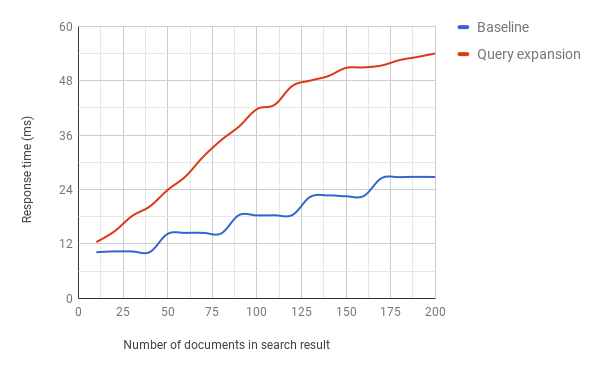
\includegraphics[width=1\linewidth]{img/result-vary-result-size.png}
  \caption{Response times using different result sizes with cache prewarming.}
  \label{fig:result-vary-result-size}
\end{figure}

\begin{figure}[h!]
  \centering 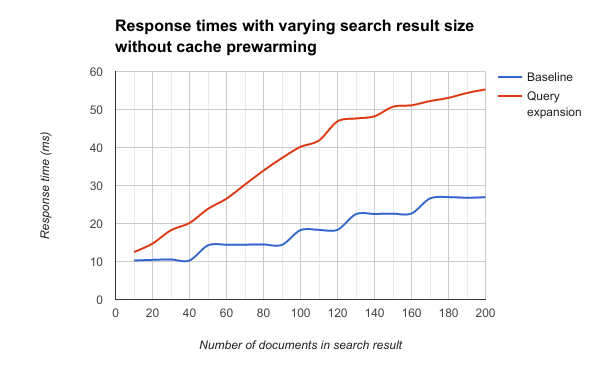
\includegraphics[width=1\linewidth]{img/result-vary-result-size-without-cache.png}
  \caption{Response times using different result sizes without cache prewarming}
  \label{fig:result-vary-result-size-without-cache}
\end{figure}
